\documentclass[10pt,a4paper]{article}
\usepackage[utf8]{inputenc}
\usepackage[T1]{fontenc}
\usepackage{lmodern}
\usepackage[margin=1in]{geometry}
\usepackage{amsmath,amssymb,amsthm}
\usepackage{booktabs}
\usepackage{graphicx}
\usepackage{microtype}
\usepackage[numbers,sort&compress]{natbib}
\usepackage{xcolor}
\usepackage[colorlinks=true,linkcolor=blue!50!black,citecolor=blue!50!black,urlcolor=blue!50!black]{hyperref}
\usepackage{enumitem}
\usepackage{array}
\usepackage{caption}
\usepackage{url}
\captionsetup{font=small,labelfont=bf}
\setlength{\textfloatsep}{9pt plus 2pt minus 2pt}
\setlength{\floatsep}{7pt plus 2pt minus 2pt}
\setlength{\intextsep}{7pt plus 2pt minus 2pt}
\renewcommand{\topfraction}{0.92}
\renewcommand{\bottomfraction}{0.6}
\renewcommand{\textfraction}{0.06}
\renewcommand{\floatpagefraction}{0.85}

\IfFileExists{numbers.tex}{% generated by experiments/make_numbers.py -- do not edit
\newcommand{\MetaSeed}{20260930}
\newcommand{\MetaPython}{3.11.15}
\newcommand{\MetaNumpy}{2.4.6}
\newcommand{\MetaScipy}{1.17.1}
\newcommand{\MetaSklearn}{1.9.1}
\newcommand{\MetaSecondsWall}{310}
\newcommand{\MetaSecondsCpu}{294}
\newcommand{\MetaMinutesCpu}{4.9}
\newcommand{\MetaSplits}{5}
\newcommand{\MetaRepeats}{5}
\newcommand{\MetaFolds}{25}
\newcommand{\MetaBoot}{10\,000}
\newcommand{\MetaCoverage}{80}
\newcommand{\MetaKgrid}{5, 10, 20, 30}
\newcommand{\MetaMgrid}{1, 2, 3, 5, 8}
\newcommand{\MetaKnnGrid}{1, 3, 5, 7, 9, 11, 15, 21, 31, 41}
\newcommand{\MetaLambdaGrid}{0.0, 0.1, 1.0, 10.0, 100.0}
\newcommand{\MetaRidge}{0.001}
\newcommand{\NDatasets}{8}
\newcommand{\NRequired}{5}
\newcommand{\NSigWins}{0}
\newcommand{\NSigLosses}{2}
\newcommand{\SigWinsList}{none}
\newcommand{\SigLossesList}{digits, moons}
\newcommand{\VerdictWord}{does not add}
\newcommand{\VerdictBool}{false}
\newcommand{\NIris}{150}
\newcommand{\DimIris}{4}
\newcommand{\ClsIris}{3}
\newcommand{\AccIrisKnn}{94.9}
\newcommand{\SdIrisKnn}{3.9}
\newcommand{\SelIrisKnn}{99.0}
\newcommand{\AccIrisNfl}{95.2}
\newcommand{\SdIrisNfl}{3.2}
\newcommand{\SelIrisNfl}{99.5}
\newcommand{\AccIrisHknn}{95.7}
\newcommand{\SdIrisHknn}{3.4}
\newcommand{\SelIrisHknn}{99.8}
\newcommand{\AccIrisLph}{96.4}
\newcommand{\SdIrisLph}{2.3}
\newcommand{\SelIrisLph}{99.7}
\newcommand{\AccIrisLcd}{95.7}
\newcommand{\SdIrisLcd}{3.5}
\newcommand{\SelIrisLcd}{99.3}
\newcommand{\AccIrisSd}{93.9}
\newcommand{\SdIrisSd}{3.9}
\newcommand{\SelIrisSd}{97.8}
\newcommand{\AccIrisTod}{96.1}
\newcommand{\SdIrisTod}{3.0}
\newcommand{\SelIrisTod}{99.3}
\newcommand{\AccIrisTo}{95.6}
\newcommand{\SdIrisTo}{3.6}
\newcommand{\SelIrisTo}{99.3}
\newcommand{\AccIrisTd}{93.6}
\newcommand{\SdIrisTd}{4.2}
\newcommand{\SelIrisTd}{98.2}
\newcommand{\AccIrisOd}{96.3}
\newcommand{\SdIrisOd}{2.8}
\newcommand{\SelIrisOd}{98.8}
\newcommand{\AccIrisT}{93.6}
\newcommand{\SdIrisT}{4.5}
\newcommand{\SelIrisT}{98.5}
\newcommand{\BestRefIris}{LPH}
\newcommand{\AccBestIris}{96.4}
\newcommand{\DeltaBestIris}{-0.3}
\newcommand{\DeltaBestTwoIris}{-0.27}
\newcommand{\CiLoBestIris}{-1.2}
\newcommand{\CiHiBestIris}{+0.7}
\newcommand{\WinsBestIris}{4/5/16}
\newcommand{\NbPBestIris}{0.834}
\newcommand{\DeltaVsIrisKnn}{+1.2}
\newcommand{\DeltaVsIrisNfl}{+0.9}
\newcommand{\DeltaVsIrisHknn}{+0.4}
\newcommand{\DeltaVsIrisLph}{-0.3}
\newcommand{\DeltaVsIrisLcd}{+0.4}
\newcommand{\DeltaVsIrisSd}{+2.3}
\newcommand{\AblIrisTo}{+0.5}
\newcommand{\AblLoIrisTo}{-0.4}
\newcommand{\AblHiIrisTo}{+1.5}
\newcommand{\AblIrisTd}{+2.5}
\newcommand{\AblLoIrisTd}{+1.3}
\newcommand{\AblHiIrisTd}{+3.7}
\newcommand{\AblIrisOd}{-0.1}
\newcommand{\AblLoIrisOd}{-1.2}
\newcommand{\AblHiIrisOd}{+0.8}
\newcommand{\AblIrisT}{+2.5}
\newcommand{\AblLoIrisT}{+1.2}
\newcommand{\AblHiIrisT}{+4.0}
\newcommand{\WTIris}{0.82}
\newcommand{\WOIris}{2.95}
\newcommand{\WDIris}{1.40}
\newcommand{\SelDeltaBestIris}{-0.3}
\newcommand{\SelCiLoIris}{-0.8}
\newcommand{\SelCiHiIris}{+0.0}
\newcommand{\NWine}{178}
\newcommand{\DimWine}{13}
\newcommand{\ClsWine}{3}
\newcommand{\AccWineKnn}{96.3}
\newcommand{\SdWineKnn}{3.4}
\newcommand{\SelWineKnn}{99.2}
\newcommand{\AccWineNfl}{97.0}
\newcommand{\SdWineNfl}{2.8}
\newcommand{\SelWineNfl}{100.0}
\newcommand{\AccWineHknn}{97.0}
\newcommand{\SdWineHknn}{2.7}
\newcommand{\SelWineHknn}{100.0}
\newcommand{\AccWineLph}{95.9}
\newcommand{\SdWineLph}{2.7}
\newcommand{\SelWineLph}{99.7}
\newcommand{\AccWineLcd}{96.9}
\newcommand{\SdWineLcd}{2.8}
\newcommand{\SelWineLcd}{99.7}
\newcommand{\AccWineSd}{96.4}
\newcommand{\SdWineSd}{3.8}
\newcommand{\SelWineSd}{98.7}
\newcommand{\AccWineTod}{97.1}
\newcommand{\SdWineTod}{2.5}
\newcommand{\SelWineTod}{99.7}
\newcommand{\AccWineTo}{96.9}
\newcommand{\SdWineTo}{2.6}
\newcommand{\SelWineTo}{100.0}
\newcommand{\AccWineTd}{96.4}
\newcommand{\SdWineTd}{3.8}
\newcommand{\SelWineTd}{98.7}
\newcommand{\AccWineOd}{97.3}
\newcommand{\SdWineOd}{3.0}
\newcommand{\SelWineOd}{99.4}
\newcommand{\AccWineT}{89.5}
\newcommand{\SdWineT}{5.7}
\newcommand{\SelWineT}{95.2}
\newcommand{\BestRefWine}{NFL}
\newcommand{\AccBestWine}{97.0}
\newcommand{\DeltaBestWine}{+0.1}
\newcommand{\DeltaBestTwoWine}{+0.10}
\newcommand{\CiLoBestWine}{-1.0}
\newcommand{\CiHiBestWine}{+1.3}
\newcommand{\WinsBestWine}{8/9/8}
\newcommand{\NbPBestWine}{0.950}
\newcommand{\DeltaVsWineKnn}{+0.8}
\newcommand{\DeltaVsWineNfl}{+0.1}
\newcommand{\DeltaVsWineHknn}{+0.1}
\newcommand{\DeltaVsWineLph}{+1.1}
\newcommand{\DeltaVsWineLcd}{+0.1}
\newcommand{\DeltaVsWineSd}{+0.7}
\newcommand{\AblWineTo}{+0.2}
\newcommand{\AblLoWineTo}{-1.0}
\newcommand{\AblHiWineTo}{+1.5}
\newcommand{\AblWineTd}{+0.7}
\newcommand{\AblLoWineTd}{-0.6}
\newcommand{\AblHiWineTd}{+2.0}
\newcommand{\AblWineOd}{-0.2}
\newcommand{\AblLoWineOd}{-1.1}
\newcommand{\AblHiWineOd}{+0.7}
\newcommand{\AblWineT}{+7.6}
\newcommand{\AblLoWineT}{+5.4}
\newcommand{\AblHiWineT}{+9.8}
\newcommand{\WTWine}{1.38}
\newcommand{\WOWine}{3.09}
\newcommand{\WDWine}{1.81}
\newcommand{\SelDeltaBestWine}{-0.3}
\newcommand{\SelCiLoWine}{-0.7}
\newcommand{\SelCiHiWine}{+0.0}
\newcommand{\NBc}{569}
\newcommand{\DimBc}{30}
\newcommand{\ClsBc}{2}
\newcommand{\AccBcKnn}{96.6}
\newcommand{\SdBcKnn}{1.7}
\newcommand{\SelBcKnn}{98.9}
\newcommand{\AccBcNfl}{96.0}
\newcommand{\SdBcNfl}{1.9}
\newcommand{\SelBcNfl}{98.8}
\newcommand{\AccBcHknn}{97.0}
\newcommand{\SdBcHknn}{1.4}
\newcommand{\SelBcHknn}{99.3}
\newcommand{\AccBcLph}{96.7}
\newcommand{\SdBcLph}{1.6}
\newcommand{\SelBcLph}{99.1}
\newcommand{\AccBcLcd}{96.9}
\newcommand{\SdBcLcd}{1.6}
\newcommand{\SelBcLcd}{99.3}
\newcommand{\AccBcSd}{95.5}
\newcommand{\SdBcSd}{1.8}
\newcommand{\SelBcSd}{98.4}
\newcommand{\AccBcTod}{96.7}
\newcommand{\SdBcTod}{1.6}
\newcommand{\SelBcTod}{99.4}
\newcommand{\AccBcTo}{97.1}
\newcommand{\SdBcTo}{1.5}
\newcommand{\SelBcTo}{99.3}
\newcommand{\AccBcTd}{95.7}
\newcommand{\SdBcTd}{1.8}
\newcommand{\SelBcTd}{98.7}
\newcommand{\AccBcOd}{96.7}
\newcommand{\SdBcOd}{1.6}
\newcommand{\SelBcOd}{99.4}
\newcommand{\AccBcT}{93.3}
\newcommand{\SdBcT}{2.0}
\newcommand{\SelBcT}{98.0}
\newcommand{\BestRefBc}{HKNN}
\newcommand{\AccBestBc}{97.0}
\newcommand{\DeltaBestBc}{-0.2}
\newcommand{\DeltaBestTwoBc}{-0.25}
\newcommand{\CiLoBestBc}{-0.7}
\newcommand{\CiHiBestBc}{+0.2}
\newcommand{\WinsBestBc}{8/11/6}
\newcommand{\NbPBestBc}{0.700}
\newcommand{\DeltaVsBcKnn}{+0.1}
\newcommand{\DeltaVsBcNfl}{+0.7}
\newcommand{\DeltaVsBcHknn}{-0.2}
\newcommand{\DeltaVsBcLph}{+0.0}
\newcommand{\DeltaVsBcLcd}{-0.1}
\newcommand{\DeltaVsBcSd}{+1.3}
\newcommand{\AblBcTo}{-0.4}
\newcommand{\AblLoBcTo}{-0.7}
\newcommand{\AblHiBcTo}{-0.0}
\newcommand{\AblBcTd}{+1.1}
\newcommand{\AblLoBcTd}{+0.5}
\newcommand{\AblHiBcTd}{+1.7}
\newcommand{\AblBcOd}{+0.0}
\newcommand{\AblLoBcOd}{-0.5}
\newcommand{\AblHiBcOd}{+0.4}
\newcommand{\AblBcT}{+3.4}
\newcommand{\AblLoBcT}{+2.7}
\newcommand{\AblHiBcT}{+4.2}
\newcommand{\WTBc}{0.71}
\newcommand{\WOBc}{2.91}
\newcommand{\WDBc}{0.89}
\newcommand{\SelDeltaBestBc}{+0.0}
\newcommand{\SelCiLoBc}{-0.2}
\newcommand{\SelCiHiBc}{+0.3}
\newcommand{\NDigits}{1000}
\newcommand{\DimDigits}{64}
\newcommand{\ClsDigits}{10}
\newcommand{\AccDigitsKnn}{96.4}
\newcommand{\SdDigitsKnn}{0.9}
\newcommand{\SelDigitsKnn}{99.3}
\newcommand{\AccDigitsNfl}{97.6}
\newcommand{\SdDigitsNfl}{1.1}
\newcommand{\SelDigitsNfl}{99.5}
\newcommand{\AccDigitsHknn}{97.4}
\newcommand{\SdDigitsHknn}{1.0}
\newcommand{\SelDigitsHknn}{99.6}
\newcommand{\AccDigitsLph}{97.4}
\newcommand{\SdDigitsLph}{0.9}
\newcommand{\SelDigitsLph}{99.5}
\newcommand{\AccDigitsLcd}{96.9}
\newcommand{\SdDigitsLcd}{1.1}
\newcommand{\SelDigitsLcd}{99.6}
\newcommand{\AccDigitsSd}{91.0}
\newcommand{\SdDigitsSd}{2.0}
\newcommand{\SelDigitsSd}{98.1}
\newcommand{\AccDigitsTod}{97.2}
\newcommand{\SdDigitsTod}{0.9}
\newcommand{\SelDigitsTod}{99.7}
\newcommand{\AccDigitsTo}{97.3}
\newcommand{\SdDigitsTo}{0.9}
\newcommand{\SelDigitsTo}{99.6}
\newcommand{\AccDigitsTd}{92.1}
\newcommand{\SdDigitsTd}{2.0}
\newcommand{\SelDigitsTd}{97.9}
\newcommand{\AccDigitsOd}{97.1}
\newcommand{\SdDigitsOd}{0.9}
\newcommand{\SelDigitsOd}{99.5}
\newcommand{\AccDigitsT}{43.6}
\newcommand{\SdDigitsT}{2.8}
\newcommand{\SelDigitsT}{47.6}
\newcommand{\BestRefDigits}{NFL}
\newcommand{\AccBestDigits}{97.6}
\newcommand{\DeltaBestDigits}{-0.3}
\newcommand{\DeltaBestTwoDigits}{-0.34}
\newcommand{\CiLoBestDigits}{-0.6}
\newcommand{\CiHiBestDigits}{-0.1}
\newcommand{\WinsBestDigits}{5/13/7}
\newcommand{\NbPBestDigits}{0.414}
\newcommand{\DeltaVsDigitsKnn}{+0.8}
\newcommand{\DeltaVsDigitsNfl}{-0.3}
\newcommand{\DeltaVsDigitsHknn}{-0.1}
\newcommand{\DeltaVsDigitsLph}{-0.2}
\newcommand{\DeltaVsDigitsLcd}{+0.4}
\newcommand{\DeltaVsDigitsSd}{+6.2}
\newcommand{\AblDigitsTo}{-0.1}
\newcommand{\AblLoDigitsTo}{-0.3}
\newcommand{\AblHiDigitsTo}{+0.1}
\newcommand{\AblDigitsTd}{+5.1}
\newcommand{\AblLoDigitsTd}{+4.4}
\newcommand{\AblHiDigitsTd}{+5.8}
\newcommand{\AblDigitsOd}{+0.1}
\newcommand{\AblLoDigitsOd}{-0.1}
\newcommand{\AblHiDigitsOd}{+0.2}
\newcommand{\AblDigitsT}{+53.6}
\newcommand{\AblLoDigitsT}{+52.5}
\newcommand{\AblHiDigitsT}{+54.7}
\newcommand{\WTDigits}{0.29}
\newcommand{\WODigits}{3.93}
\newcommand{\WDDigits}{0.52}
\newcommand{\SelDeltaBestDigits}{+0.2}
\newcommand{\SelCiLoDigits}{+0.0}
\newcommand{\SelCiHiDigits}{+0.3}
\newcommand{\NSwiss}{600}
\newcommand{\DimSwiss}{3}
\newcommand{\ClsSwiss}{3}
\newcommand{\AccSwissKnn}{96.8}
\newcommand{\SdSwissKnn}{1.8}
\newcommand{\SelSwissKnn}{99.5}
\newcommand{\AccSwissNfl}{92.9}
\newcommand{\SdSwissNfl}{2.4}
\newcommand{\SelSwissNfl}{98.0}
\newcommand{\AccSwissHknn}{97.4}
\newcommand{\SdSwissHknn}{1.1}
\newcommand{\SelSwissHknn}{99.6}
\newcommand{\AccSwissLph}{97.0}
\newcommand{\SdSwissLph}{1.9}
\newcommand{\SelSwissLph}{99.6}
\newcommand{\AccSwissLcd}{96.9}
\newcommand{\SdSwissLcd}{1.4}
\newcommand{\SelSwissLcd}{99.7}
\newcommand{\AccSwissSd}{95.4}
\newcommand{\SdSwissSd}{2.1}
\newcommand{\SelSwissSd}{99.0}
\newcommand{\AccSwissTod}{97.2}
\newcommand{\SdSwissTod}{1.7}
\newcommand{\SelSwissTod}{99.5}
\newcommand{\AccSwissTo}{97.2}
\newcommand{\SdSwissTo}{1.9}
\newcommand{\SelSwissTo}{99.5}
\newcommand{\AccSwissTd}{95.2}
\newcommand{\SdSwissTd}{1.8}
\newcommand{\SelSwissTd}{98.8}
\newcommand{\AccSwissOd}{97.1}
\newcommand{\SdSwissOd}{1.8}
\newcommand{\SelSwissOd}{99.5}
\newcommand{\AccSwissT}{78.9}
\newcommand{\SdSwissT}{3.8}
\newcommand{\SelSwissT}{84.0}
\newcommand{\BestRefSwiss}{HKNN}
\newcommand{\AccBestSwiss}{97.4}
\newcommand{\DeltaBestSwiss}{-0.2}
\newcommand{\DeltaBestTwoSwiss}{-0.20}
\newcommand{\CiLoBestSwiss}{-0.6}
\newcommand{\CiHiBestSwiss}{+0.2}
\newcommand{\WinsBestSwiss}{7/9/9}
\newcommand{\NbPBestSwiss}{0.721}
\newcommand{\DeltaVsSwissKnn}{+0.3}
\newcommand{\DeltaVsSwissNfl}{+4.3}
\newcommand{\DeltaVsSwissHknn}{-0.2}
\newcommand{\DeltaVsSwissLph}{+0.2}
\newcommand{\DeltaVsSwissLcd}{+0.3}
\newcommand{\DeltaVsSwissSd}{+1.8}
\newcommand{\AblSwissTo}{-0.1}
\newcommand{\AblLoSwissTo}{-0.4}
\newcommand{\AblHiSwissTo}{+0.3}
\newcommand{\AblSwissTd}{+1.9}
\newcommand{\AblLoSwissTd}{+1.2}
\newcommand{\AblHiSwissTd}{+2.7}
\newcommand{\AblSwissOd}{+0.1}
\newcommand{\AblLoSwissOd}{-0.4}
\newcommand{\AblHiSwissOd}{+0.5}
\newcommand{\AblSwissT}{+18.3}
\newcommand{\AblLoSwissT}{+16.8}
\newcommand{\AblHiSwissT}{+19.9}
\newcommand{\WTSwiss}{0.17}
\newcommand{\WOSwiss}{3.30}
\newcommand{\WDSwiss}{0.57}
\newcommand{\SelDeltaBestSwiss}{-0.1}
\newcommand{\SelCiLoSwiss}{-0.2}
\newcommand{\SelCiHiSwiss}{+0.1}
\newcommand{\NMoons}{600}
\newcommand{\DimMoons}{2}
\newcommand{\ClsMoons}{2}
\newcommand{\AccMoonsKnn}{89.9}
\newcommand{\SdMoonsKnn}{2.8}
\newcommand{\SelMoonsKnn}{95.2}
\newcommand{\AccMoonsNfl}{80.0}
\newcommand{\SdMoonsNfl}{3.9}
\newcommand{\SelMoonsNfl}{85.1}
\newcommand{\AccMoonsHknn}{89.9}
\newcommand{\SdMoonsHknn}{2.9}
\newcommand{\SelMoonsHknn}{93.8}
\newcommand{\AccMoonsLph}{88.9}
\newcommand{\SdMoonsLph}{3.3}
\newcommand{\SelMoonsLph}{92.8}
\newcommand{\AccMoonsLcd}{89.9}
\newcommand{\SdMoonsLcd}{2.9}
\newcommand{\SelMoonsLcd}{96.0}
\newcommand{\AccMoonsSd}{88.6}
\newcommand{\SdMoonsSd}{2.9}
\newcommand{\SelMoonsSd}{91.4}
\newcommand{\AccMoonsTod}{89.1}
\newcommand{\SdMoonsTod}{3.3}
\newcommand{\SelMoonsTod}{92.8}
\newcommand{\AccMoonsTo}{89.1}
\newcommand{\SdMoonsTo}{3.3}
\newcommand{\SelMoonsTo}{92.8}
\newcommand{\AccMoonsTd}{88.0}
\newcommand{\SdMoonsTd}{2.8}
\newcommand{\SelMoonsTd}{92.0}
\newcommand{\AccMoonsOd}{89.0}
\newcommand{\SdMoonsOd}{3.5}
\newcommand{\SelMoonsOd}{92.9}
\newcommand{\AccMoonsT}{78.7}
\newcommand{\SdMoonsT}{4.2}
\newcommand{\SelMoonsT}{83.7}
\newcommand{\BestRefMoons}{HKNN}
\newcommand{\AccBestMoons}{89.9}
\newcommand{\DeltaBestMoons}{-0.8}
\newcommand{\DeltaBestTwoMoons}{-0.77}
\newcommand{\CiLoBestMoons}{-1.3}
\newcommand{\CiHiBestMoons}{-0.3}
\newcommand{\WinsBestMoons}{5/16/4}
\newcommand{\NbPBestMoons}{0.290}
\newcommand{\DeltaVsMoonsKnn}{-0.8}
\newcommand{\DeltaVsMoonsNfl}{+9.2}
\newcommand{\DeltaVsMoonsHknn}{-0.8}
\newcommand{\DeltaVsMoonsLph}{+0.2}
\newcommand{\DeltaVsMoonsLcd}{-0.8}
\newcommand{\DeltaVsMoonsSd}{+0.5}
\newcommand{\AblMoonsTo}{+0.0}
\newcommand{\AblLoMoonsTo}{-0.4}
\newcommand{\AblHiMoonsTo}{+0.4}
\newcommand{\AblMoonsTd}{+1.1}
\newcommand{\AblLoMoonsTd}{+0.2}
\newcommand{\AblHiMoonsTd}{+2.0}
\newcommand{\AblMoonsOd}{+0.1}
\newcommand{\AblLoMoonsOd}{-0.3}
\newcommand{\AblHiMoonsOd}{+0.6}
\newcommand{\AblMoonsT}{+10.5}
\newcommand{\AblLoMoonsT}{+8.4}
\newcommand{\AblHiMoonsT}{+12.5}
\newcommand{\WTMoons}{0.42}
\newcommand{\WOMoons}{1.52}
\newcommand{\WDMoons}{-0.12}
\newcommand{\SelDeltaBestMoons}{-1.0}
\newcommand{\SelCiLoMoons}{-1.6}
\newcommand{\SelCiHiMoons}{-0.5}
\newcommand{\NMoonsN}{600}
\newcommand{\DimMoonsN}{12}
\newcommand{\ClsMoonsN}{2}
\newcommand{\AccMoonsNKnn}{82.8}
\newcommand{\SdMoonsNKnn}{3.4}
\newcommand{\SelMoonsNKnn}{88.3}
\newcommand{\AccMoonsNNfl}{77.7}
\newcommand{\SdMoonsNNfl}{2.8}
\newcommand{\SelMoonsNNfl}{82.2}
\newcommand{\AccMoonsNHknn}{82.8}
\newcommand{\SdMoonsNHknn}{3.3}
\newcommand{\SelMoonsNHknn}{88.5}
\newcommand{\AccMoonsNLph}{82.1}
\newcommand{\SdMoonsNLph}{3.2}
\newcommand{\SelMoonsNLph}{87.7}
\newcommand{\AccMoonsNLcd}{82.8}
\newcommand{\SdMoonsNLcd}{4.2}
\newcommand{\SelMoonsNLcd}{88.9}
\newcommand{\AccMoonsNSd}{80.0}
\newcommand{\SdMoonsNSd}{3.3}
\newcommand{\SelMoonsNSd}{85.9}
\newcommand{\AccMoonsNTod}{82.5}
\newcommand{\SdMoonsNTod}{3.3}
\newcommand{\SelMoonsNTod}{87.5}
\newcommand{\AccMoonsNTo}{82.6}
\newcommand{\SdMoonsNTo}{3.2}
\newcommand{\SelMoonsNTo}{87.5}
\newcommand{\AccMoonsNTd}{79.8}
\newcommand{\SdMoonsNTd}{3.4}
\newcommand{\SelMoonsNTd}{85.8}
\newcommand{\AccMoonsNOd}{81.9}
\newcommand{\SdMoonsNOd}{3.1}
\newcommand{\SelMoonsNOd}{87.8}
\newcommand{\AccMoonsNT}{62.8}
\newcommand{\SdMoonsNT}{4.7}
\newcommand{\SelMoonsNT}{64.9}
\newcommand{\BestRefMoonsN}{HKNN}
\newcommand{\AccBestMoonsN}{82.8}
\newcommand{\DeltaBestMoonsN}{-0.4}
\newcommand{\DeltaBestTwoMoonsN}{-0.37}
\newcommand{\CiLoBestMoonsN}{-1.3}
\newcommand{\CiHiBestMoonsN}{+0.6}
\newcommand{\WinsBestMoonsN}{10/11/4}
\newcommand{\NbPBestMoonsN}{0.779}
\newcommand{\DeltaVsMoonsNKnn}{-0.3}
\newcommand{\DeltaVsMoonsNNfl}{+4.8}
\newcommand{\DeltaVsMoonsNHknn}{-0.4}
\newcommand{\DeltaVsMoonsNLph}{+0.3}
\newcommand{\DeltaVsMoonsNLcd}{-0.4}
\newcommand{\DeltaVsMoonsNSd}{+2.5}
\newcommand{\AblMoonsNTo}{-0.2}
\newcommand{\AblLoMoonsNTo}{-1.1}
\newcommand{\AblHiMoonsNTo}{+0.7}
\newcommand{\AblMoonsNTd}{+2.7}
\newcommand{\AblLoMoonsNTd}{+1.5}
\newcommand{\AblHiMoonsNTd}{+3.8}
\newcommand{\AblMoonsNOd}{+0.5}
\newcommand{\AblLoMoonsNOd}{-0.4}
\newcommand{\AblHiMoonsNOd}{+1.5}
\newcommand{\AblMoonsNT}{+19.7}
\newcommand{\AblLoMoonsNT}{+17.6}
\newcommand{\AblHiMoonsNT}{+21.7}
\newcommand{\WTMoonsN}{0.37}
\newcommand{\WOMoonsN}{3.04}
\newcommand{\WDMoonsN}{-1.15}
\newcommand{\SelDeltaBestMoonsN}{-1.0}
\newcommand{\SelCiLoMoonsN}{-1.7}
\newcommand{\SelCiHiMoonsN}{-0.3}
\newcommand{\NSpheres}{600}
\newcommand{\DimSpheres}{3}
\newcommand{\ClsSpheres}{2}
\newcommand{\AccSpheresKnn}{82.5}
\newcommand{\SdSpheresKnn}{3.1}
\newcommand{\SelSpheresKnn}{88.0}
\newcommand{\AccSpheresNfl}{78.6}
\newcommand{\SdSpheresNfl}{2.9}
\newcommand{\SelSpheresNfl}{83.3}
\newcommand{\AccSpheresHknn}{85.5}
\newcommand{\SdSpheresHknn}{3.2}
\newcommand{\SelSpheresHknn}{90.9}
\newcommand{\AccSpheresLph}{84.8}
\newcommand{\SdSpheresLph}{3.2}
\newcommand{\SelSpheresLph}{89.9}
\newcommand{\AccSpheresLcd}{83.5}
\newcommand{\SdSpheresLcd}{3.3}
\newcommand{\SelSpheresLcd}{89.1}
\newcommand{\AccSpheresSd}{81.9}
\newcommand{\SdSpheresSd}{2.2}
\newcommand{\SelSpheresSd}{86.4}
\newcommand{\AccSpheresTod}{85.7}
\newcommand{\SdSpheresTod}{3.4}
\newcommand{\SelSpheresTod}{90.8}
\newcommand{\AccSpheresTo}{85.2}
\newcommand{\SdSpheresTo}{3.4}
\newcommand{\SelSpheresTo}{90.0}
\newcommand{\AccSpheresTd}{82.2}
\newcommand{\SdSpheresTd}{2.1}
\newcommand{\SelSpheresTd}{86.4}
\newcommand{\AccSpheresOd}{85.8}
\newcommand{\SdSpheresOd}{2.4}
\newcommand{\SelSpheresOd}{90.5}
\newcommand{\AccSpheresT}{70.8}
\newcommand{\SdSpheresT}{4.4}
\newcommand{\SelSpheresT}{75.0}
\newcommand{\BestRefSpheres}{HKNN}
\newcommand{\AccBestSpheres}{85.5}
\newcommand{\DeltaBestSpheres}{+0.2}
\newcommand{\DeltaBestTwoSpheres}{+0.23}
\newcommand{\CiLoBestSpheres}{-0.5}
\newcommand{\CiHiBestSpheres}{+1.0}
\newcommand{\WinsBestSpheres}{11/10/4}
\newcommand{\NbPBestSpheres}{0.824}
\newcommand{\DeltaVsSpheresKnn}{+3.2}
\newcommand{\DeltaVsSpheresNfl}{+7.1}
\newcommand{\DeltaVsSpheresHknn}{+0.2}
\newcommand{\DeltaVsSpheresLph}{+0.9}
\newcommand{\DeltaVsSpheresLcd}{+2.2}
\newcommand{\DeltaVsSpheresSd}{+3.8}
\newcommand{\AblSpheresTo}{+0.5}
\newcommand{\AblLoSpheresTo}{-0.0}
\newcommand{\AblHiSpheresTo}{+1.0}
\newcommand{\AblSpheresTd}{+3.5}
\newcommand{\AblLoSpheresTd}{+2.3}
\newcommand{\AblHiSpheresTd}{+4.7}
\newcommand{\AblSpheresOd}{-0.1}
\newcommand{\AblLoSpheresOd}{-0.9}
\newcommand{\AblHiSpheresOd}{+0.7}
\newcommand{\AblSpheresT}{+14.9}
\newcommand{\AblLoSpheresT}{+13.1}
\newcommand{\AblHiSpheresT}{+16.7}
\newcommand{\WTSpheres}{0.26}
\newcommand{\WOSpheres}{1.92}
\newcommand{\WDSpheres}{-0.53}
\newcommand{\SelDeltaBestSpheres}{-0.1}
\newcommand{\SelCiLoSpheres}{-0.8}
\newcommand{\SelCiHiSpheres}{+0.5}
\newcommand{\DeltaBestMin}{-0.8}
\newcommand{\DeltaBestMax}{+0.2}
\newcommand{\DeltaBestAbsMax}{0.8}
\newcommand{\NDeltaWithinOne}{8}
\newcommand{\NDeltaWithinHalf}{7}
\newcommand{\DeltaHknnMin}{-0.8}
\newcommand{\DeltaHknnMax}{+0.4}
\newcommand{\NHknnCiAboveZero}{0}
\newcommand{\NHknnCiBelowZero}{1}
\newcommand{\DeltaLphMin}{-0.3}
\newcommand{\DeltaLphMax}{+1.1}
\newcommand{\NLphCiAboveZero}{1}
\newcommand{\DeltaSdMin}{+0.5}
\newcommand{\DeltaSdMax}{+6.2}
\newcommand{\NSdCiAboveZero}{6}
\newcommand{\DeltaKnnMin}{-0.8}
\newcommand{\DeltaKnnMax}{+3.2}
\newcommand{\NKnnCiAboveZero}{2}
\newcommand{\NKnnCiBelowZero}{0}
\newcommand{\AblDepthMin}{-0.4}
\newcommand{\AblDepthMax}{+0.5}
\newcommand{\NAblDepthCiAboveZero}{0}
\newcommand{\NAblDepthCiBelowZero}{1}
\newcommand{\AblDepthArgMax}{iris}
\newcommand{\AblOrthMin}{+0.7}
\newcommand{\AblOrthMax}{+5.1}
\newcommand{\NAblOrthCiAboveZero}{7}
\newcommand{\NAblOrthCiBelowZero}{0}
\newcommand{\AblOrthArgMax}{digits}
\newcommand{\AblTangMin}{-0.2}
\newcommand{\AblTangMax}{+0.5}
\newcommand{\NAblTangCiAboveZero}{0}
\newcommand{\NAblTangCiBelowZero}{0}
\newcommand{\AblTangArgMax}{moons+10 noise}
\newcommand{\SelDeltaMin}{-1.0}
\newcommand{\SelDeltaMax}{+0.2}
\newcommand{\NSelCiAboveZero}{1}
\newcommand{\NSelCiBelowZero}{2}
\newcommand{\WDMin}{-1.15}
\newcommand{\WDMax}{1.81}
\newcommand{\WOMin}{1.52}
\newcommand{\WOMax}{3.93}
\newcommand{\WTMin}{0.17}
\newcommand{\WTMax}{1.38}
\newcommand{\NBestRefHull}{8}
\newcommand{\NBestRefKnn}{0}
\newcommand{\NBestRefLcd}{0}
\newcommand{\NBestRefSd}{0}
\newcommand{\BestRefSet}{HKNN, LPH, NFL}
\newcommand{\HullFamilyMaxSpread}{1.3}
\newcommand{\AccTMin}{43.6}
\newcommand{\AccTMax}{93.6}
\newcommand{\AccTArgMin}{digits}
\newcommand{\CiHiBestMax}{+1.3}
\newcommand{\CiHiHknnMax}{+1.3}
\newcommand{\CiHiLphMax}{+2.4}
\newcommand{\AblDepthCiHiMax}{+1.5}
\newcommand{\AblTangCiHiMax}{+1.5}
\newcommand{\NWDNegative}{3}
\newcommand{\NHknnLambdaMax}{1}
\newcommand{\NKnnKMax}{2}
\newcommand{\NLocalKMax}{3}
\newcommand{\RegPZeroKnn}{89.9}
\newcommand{\RegPZeroNfl}{80.0}
\newcommand{\RegPZeroHknn}{89.9}
\newcommand{\RegPZeroLph}{88.9}
\newcommand{\RegPZeroLcd}{89.9}
\newcommand{\RegPZeroSd}{88.6}
\newcommand{\RegPZeroTod}{89.1}
\newcommand{\RegPZeroTo}{89.1}
\newcommand{\RegPZeroTd}{88.0}
\newcommand{\RegPZeroOd}{89.0}
\newcommand{\RegPZeroT}{78.7}
\newcommand{\RegBestPZero}{HKNN}
\newcommand{\RegDeltaPZero}{-0.8}
\newcommand{\RegLoPZero}{-1.3}
\newcommand{\RegHiPZero}{-0.3}
\newcommand{\RegAblDepthPZero}{+0.0}
\newcommand{\RegAblDepthLoPZero}{-0.4}
\newcommand{\RegAblDepthHiPZero}{+0.4}
\newcommand{\RegBestAccPZero}{89.9}
\newcommand{\RegAblTangPZero}{+0.1}
\newcommand{\RegPTwoKnn}{87.1}
\newcommand{\RegPTwoNfl}{82.6}
\newcommand{\RegPTwoHknn}{86.4}
\newcommand{\RegPTwoLph}{86.9}
\newcommand{\RegPTwoLcd}{87.9}
\newcommand{\RegPTwoSd}{85.5}
\newcommand{\RegPTwoTod}{87.8}
\newcommand{\RegPTwoTo}{86.9}
\newcommand{\RegPTwoTd}{85.5}
\newcommand{\RegPTwoOd}{87.5}
\newcommand{\RegPTwoT}{78.5}
\newcommand{\RegBestPTwo}{LCD}
\newcommand{\RegDeltaPTwo}{-0.1}
\newcommand{\RegLoPTwo}{-0.7}
\newcommand{\RegHiPTwo}{+0.6}
\newcommand{\RegAblDepthPTwo}{+0.9}
\newcommand{\RegAblDepthLoPTwo}{+0.3}
\newcommand{\RegAblDepthHiPTwo}{+1.5}
\newcommand{\RegBestAccPTwo}{87.9}
\newcommand{\RegAblTangPTwo}{+0.3}
\newcommand{\RegPFiveKnn}{84.4}
\newcommand{\RegPFiveNfl}{81.9}
\newcommand{\RegPFiveHknn}{83.9}
\newcommand{\RegPFiveLph}{83.9}
\newcommand{\RegPFiveLcd}{84.9}
\newcommand{\RegPFiveSd}{82.3}
\newcommand{\RegPFiveTod}{84.6}
\newcommand{\RegPFiveTo}{84.0}
\newcommand{\RegPFiveTd}{82.5}
\newcommand{\RegPFiveOd}{84.3}
\newcommand{\RegPFiveT}{67.7}
\newcommand{\RegBestPFive}{LCD}
\newcommand{\RegDeltaPFive}{-0.3}
\newcommand{\RegLoPFive}{-0.9}
\newcommand{\RegHiPFive}{+0.4}
\newcommand{\RegAblDepthPFive}{+0.6}
\newcommand{\RegAblDepthLoPFive}{-0.2}
\newcommand{\RegAblDepthHiPFive}{+1.5}
\newcommand{\RegBestAccPFive}{84.9}
\newcommand{\RegAblTangPFive}{+0.3}
\newcommand{\RegPTenKnn}{82.8}
\newcommand{\RegPTenNfl}{77.7}
\newcommand{\RegPTenHknn}{82.8}
\newcommand{\RegPTenLph}{82.1}
\newcommand{\RegPTenLcd}{82.8}
\newcommand{\RegPTenSd}{80.0}
\newcommand{\RegPTenTod}{82.5}
\newcommand{\RegPTenTo}{82.6}
\newcommand{\RegPTenTd}{79.8}
\newcommand{\RegPTenOd}{81.9}
\newcommand{\RegPTenT}{62.8}
\newcommand{\RegBestPTen}{HKNN}
\newcommand{\RegDeltaPTen}{-0.4}
\newcommand{\RegLoPTen}{-1.3}
\newcommand{\RegHiPTen}{+0.5}
\newcommand{\RegAblDepthPTen}{-0.2}
\newcommand{\RegAblDepthLoPTen}{-1.1}
\newcommand{\RegAblDepthHiPTen}{+0.8}
\newcommand{\RegBestAccPTen}{82.8}
\newcommand{\RegAblTangPTen}{+0.5}
\newcommand{\RegPTwentyKnn}{80.9}
\newcommand{\RegPTwentyNfl}{75.7}
\newcommand{\RegPTwentyHknn}{81.4}
\newcommand{\RegPTwentyLph}{80.6}
\newcommand{\RegPTwentyLcd}{81.3}
\newcommand{\RegPTwentySd}{79.1}
\newcommand{\RegPTwentyTod}{81.0}
\newcommand{\RegPTwentyTo}{81.1}
\newcommand{\RegPTwentyTd}{78.7}
\newcommand{\RegPTwentyOd}{80.8}
\newcommand{\RegPTwentyT}{51.2}
\newcommand{\RegBestPTwenty}{HKNN}
\newcommand{\RegDeltaPTwenty}{-0.4}
\newcommand{\RegLoPTwenty}{-1.2}
\newcommand{\RegHiPTwenty}{+0.3}
\newcommand{\RegAblDepthPTwenty}{-0.1}
\newcommand{\RegAblDepthLoPTwenty}{-0.7}
\newcommand{\RegAblDepthHiPTwenty}{+0.5}
\newcommand{\RegBestAccPTwenty}{81.4}
\newcommand{\RegAblTangPTwenty}{+0.2}
\newcommand{\NRegSigWins}{0}
\newcommand{\NRegSigLosses}{1}
\newcommand{\NRegime}{5}
\newcommand{\RegDeltaMin}{-0.8}
\newcommand{\RegDeltaMax}{-0.1}
\newcommand{\RegBestSet}{HKNN, LCD}
\newcommand{\RegAblDepthMin}{-0.2}
\newcommand{\RegAblDepthMax}{+0.9}
\newcommand{\RegAblTangMin}{+0.1}
\newcommand{\RegAblTangMax}{+0.5}
\newcommand{\RegAblOrthMin}{+1.1}
\newcommand{\RegAblOrthMax}{+2.7}
\newcommand{\NRegAblDepthCiAboveZero}{1}
\newcommand{\NRegAblTangCiAboveZero}{0}
\newcommand{\RegSdDrop}{9.5}
\newcommand{\RegKnnDrop}{9.0}
\newcommand{\RegTodDrop}{8.2}
\newcommand{\RegHknnDrop}{8.5}
}{}

\theoremstyle{plain}
\newtheorem{theorem}{Theorem}[section]
\newtheorem{proposition}[theorem]{Proposition}
\newtheorem{lemma}[theorem]{Lemma}
\newtheorem{corollary}[theorem]{Corollary}
\theoremstyle{definition}
\newtheorem{definition}[theorem]{Definition}
\newtheorem{example}[theorem]{Example}
\theoremstyle{remark}
\newtheorem{remark}[theorem]{Remark}

\newcommand{\R}{\mathbb{R}}
\newcommand{\Nk}{N_k^{c}(q)}
\newcommand{\aff}{\operatorname{aff}}
\newcommand{\dist}{\operatorname{dist}}
\newcommand{\status}[1]{\textsf{\small [#1]}}
\newcommand{\meth}[1]{\textsf{#1}}
\newcommand{\kNN}{k_{\rm NN}}

\title{\textbf{Support Geometry and Nearest Neighbours:}\\[2pt]
\large Does the Tangential--Orthogonal--Depth Decomposition Add Information\\ Beyond Feature Lines, Local Hulls and Depth?}
\author{Luciano Silva Alarco\\
\small Pontificia Universidad Cat\'olica del Per\'u\\
\small ORCID 0000-0002-3395-3129}
\date{\small Working draft v0.2 (round 1 of internal review applied) --- research line SPD001 --- 3 October 2026}

\begin{document}
\maketitle

\begin{abstract}
\noindent
For a query $q$ and its $k$ nearest training neighbours of a class, the residual from the neighbourhood centroid splits into a \emph{tangential} component along the local principal subspace and an \emph{orthogonal} component normal to it, and the position of $q$ among the neighbours can be summarised by a \emph{depth}. The research line SPD001 asked whether this description carries information for classification beyond nearest feature lines, local hulls and depth measures. We show that the regularised local-hyperplane distance of Vincent and Bengio is exactly a data-weighted sum of the orthogonal component and the squared tangential coordinates, $h_\lambda^2=O^2+\sum_j \lambda t_j^2/(s_j^2+\lambda)$, while the local spatial depth is not a function of the two distances. We then run the isolating comparison the line had left pending (\NDatasets{} datasets, $\MetaSplits\times\MetaRepeats$ repeated cross-validation, six tuned references, a conditional-logit combination of the three components and its ablations) under a criterion fixed before the first complete run: a paired bootstrap interval above zero against the best reference on at least \NRequired{} of \NDatasets{} datasets. The combination met it on \NSigWins; its difference to the best reference ranged from \DeltaBestMin{} to \DeltaBestMax{} accuracy points, and the largest upper limit is \CiHiBestMax{} points with the bootstrap and \CiHiBestMaxNb{} with the Nadeau--Bengio variance, so the study excludes gains of a few points, not of one. Removing the orthogonal component costs \AblOrthMin{} to \AblOrthMax{} points (interval above zero on \NAblOrthCiAboveZero{} of \NDatasets{} datasets with the bootstrap, \NAblOrthNbAboveZero{} with Nadeau--Bengio); removing the depth or the tangential component never does so significantly. The decomposition describes local-hull classifiers well, but it does not add predictive information beyond them.
\end{abstract}

\section{Introduction}\label{sec:intro}

Nearest-neighbour classification~\citep{fixhodges1989,coverhart1967} uses only distances from the query to individual training points. A family of extensions replaces the point by a local set built from the query's neighbours in each class: the line through two prototypes (nearest feature line, \citealp{lilu1999}), the affine hull of the $k$ nearest same-class neighbours with a ridge penalty (HKNN, \citealp{vincentbengio2002}), bounded hulls and hyperdisks~\citep{cevikalp2008}, local principal subspaces~\citep{kambhatlaleen1997} or locally adapted metrics~\citep{hastietibshirani1996}. All of them measure, in one way or another, how far the query lies \emph{off} the local class support. A separate tradition, statistical depth~\citep{tukey1975,liu1990,zuoserfling2000}, measures how central a point is \emph{inside} a cloud, and depth-based classifiers assign the query to the class in which it is deepest~\citep{ghoshchaudhuri2005,licuestaliu2012}, with local versions for multimodal classes~\citep{paindaveinevanbever2013}.

The research line SPD001 (``support geometry and nearest neighbours'') set out from the observation that these quantities are components of one decomposition: if $\mu$ is the centroid of the $k$ nearest neighbours of $q$ in class $c$ and $T_m$ the $m$-dimensional principal subspace of that neighbourhood, $q-\mu$ splits orthogonally into a tangential part in $T_m$ and an orthogonal part normal to it, and a depth measures where $q$ falls relative to the neighbours. The line's public record states its objective as \emph{determining whether this decomposition adds information beyond feature lines, hulls and depth measures}, and its findings as \emph{a comparison isolating a specific contribution remains pending; no improvement in predictive accuracy has been validated}. This paper runs that comparison and writes down the answer, with the elementary facts that explain it.

\paragraph{Contributions.} (i)~Precise definitions of the tangential, orthogonal and depth components of a query with respect to a class neighbourhood (Section~\ref{sec:defs}). (ii)~Elementary propositions (Section~\ref{sec:theory}): the regularised HKNN distance is an explicit weighted combination of the orthogonal component and the tangential coordinates, monotone in the penalty and bounded by the hull distance and the centroid distance; the nearest-feature-line distance restricted to the same neighbours is sandwiched between the hull distance and the nearest-neighbour distance; the local spatial depth is not a function of the two distances, so it \emph{could} carry information. (iii)~The isolating comparison with a criterion stated before the first complete run (Section~\ref{sec:protocol}) and its outcome (Section~\ref{sec:results}), which is negative under that criterion. (iv)~A list of claims with their status (Section~\ref{sec:claims}).

\paragraph{Scope.} The paper is a methodological study on small public and synthetic datasets; it makes no claim about any application domain. ``Adds information'' is given one operational meaning (Section~\ref{sec:protocol}); other meanings, such as usefulness for visualisation or description, are not tested and not denied. Every number is produced by the scripts of Appendix~\ref{app:repro} with a fixed seed; none is typed by hand.

\section{Definitions}\label{sec:defs}

Let $(x_i,y_i)_{i=1}^n$ be a training set with $x_i\in\R^d$ and labels $y_i\in\{1,\dots,C\}$, standardised coordinate-wise with training statistics. Fix a query $q\in\R^d$, a class $c$ and an integer $k$ with $k\le n_c$, where $n_c$ is the number of training points of class $c$ (when $q$ is itself a training point it is excluded from its own neighbourhoods).

\begin{definition}[class neighbourhood, centred SVD]\label{def:nbhd}
$\Nk\subset\{x_i: y_i=c\}$ is the set of the $k$ training points of class $c$ nearest to $q$ in Euclidean distance (ties broken deterministically). Let $\mu=\mu_c(q)$ be its mean, $V\in\R^{k\times d}$ the matrix with rows $x_i-\mu$, $x_i\in\Nk$, and $V=W\,\mathrm{diag}(s_1,\dots,s_p)\,U^{\top}$ a thin singular value decomposition with $p=\min(k,d)$, $s_1\ge\dots\ge s_p\ge0$ and orthonormal columns $u_1,\dots,u_p$ of $U$. Write $r=q-\mu$ and $t_j=u_j^{\top}r$. Since the rows of $V$ sum to zero, $\operatorname{rank}V\le\min(k-1,d)$; we call the neighbourhood \emph{generic} when equality holds, and write $\rho=\min(k-1,d)$.
\end{definition}

\begin{definition}[tangential and orthogonal components]\label{def:TO}\sloppy
For $1\le m\le\rho$ let $T_m=\operatorname{span}(u_1,\dots,u_m)$ (the local principal, or tangent, subspace of dimension $m$) and $P_m$ the orthogonal projector onto it. The \emph{tangential distance} and the \emph{orthogonal distance} of $q$ to the class-$c$ neighbourhood are
\[
T_m(q,c)=\|P_m r\|=\Big(\sum_{j\le m}t_j^2\Big)^{1/2},\qquad
O_m(q,c)=\|(I-P_m)r\|=\Big(\|r\|^2-\sum_{j\le m}t_j^2\Big)^{1/2}.
\]
\end{definition}

\begin{definition}[local hull, HKNN and feature-line distances]\label{def:hull}
The \emph{local hull distance} is $\dist(q,\aff\Nk)$, the Euclidean distance from $q$ to the affine hull of the neighbourhood. For $\lambda\ge0$ the \emph{penalised local-hyperplane distance} of \citet{vincentbengio2002} is
\[
h_\lambda(q,c)^2=\min_{\alpha\in\R^k}\ \|r-V^{\top}\alpha\|^2+\lambda\|\alpha\|^2 .
\]
We take as the \meth{HKNN} score the value of this penalised objective; this is our reading of Section~3 of \citet{vincentbengio2002}. If one takes instead the plain distance $\|r-V^{\top}\alpha^*\|$ at the penalised minimiser $\alpha^*$, Proposition~\ref{prop:hknn} below holds with weights $\lambda^2/(s_j^2+\lambda)^2$ in place of $\lambda/(s_j^2+\lambda)$, and nothing else in the paper changes. The \emph{local feature-line distance} is $\ell(q,c)=\min_{x_i\ne x_j\in\Nk}\dist\big(q,\,x_i+\R(x_j-x_i)\big)$, the nearest-feature-line distance of \citet{lilu1999} restricted to the $k$ neighbours. The \emph{local class distance} is $\bar d(q,c)=\frac1k\sum_{x_i\in\Nk}\|q-x_i\|$.
\end{definition}

\begin{definition}[local spatial depth]\label{def:depth}
With the spatial sign $S(v)=v/\|v\|$ for $v\ne0$ and $S(0)=0$, the \emph{local spatial depth} of $q$ with respect to the class-$c$ neighbourhood is
\[
D(q,c)=1-\Big\|\frac1k\sum_{x_i\in\Nk}S(x_i-q)\Big\|\in[0,1],
\]
the spatial ($L_1$) depth of \citet{vardizhang2000} and \citet{serfling2002}, computed on the neighbourhood instead of on the whole class. We call $E=1-D$ the \emph{outlyingness}.
\end{definition}

The spatial depth equals $1$ at the spatial median of the neighbourhood when the median is not itself a neighbour (at a neighbour $x_i$ the term $S(0)=0$ drops out and $D(x_i)$ may be below $1$); the median is unique when the neighbours are not collinear~\citep{milasevicducharme1987}; $D$ tends to $0$ as $\|q\|\to\infty$ and is invariant under orthogonal transformations and translations but not under general affine maps~\citep{chaudhuri1996,vardizhang2000,serfling2002} \status{literature}. Restricting a depth to a neighbourhood of the query is a simple proxy for the local depths of \citet{paindaveinevanbever2013}; we do not use their symmetrised construction.

\begin{definition}[classifiers]\label{def:clf}\sloppy
All classifiers below assign $q$ to the class that minimises a score $\sigma(q,c)$ (or maximises the depth), with no class prior, except \meth{kNN}, which takes a majority vote among the $\kNN$ nearest neighbours of all classes (ties towards the class of the nearest neighbour).
\begin{itemize}[leftmargin=2em,itemsep=1pt]
\item \meth{NFL}: $\sigma=\ell(q,c)$;\quad \meth{HKNN}: $\sigma=h_\lambda(q,c)$;\quad \meth{LPH} (local PCA hull): $\sigma=O_m(q,c)$;
\item \meth{LCD}: $\sigma=\bar d(q,c)$;\quad \meth{SD}: $\sigma=E(q,c)$;\quad \meth{T}: $\sigma=T_m(q,c)$;
\item \meth{TOD} (the decomposition classifier): with the feature vector $f_c(q)=\big(\log T_m,\ \log O_m,\ \log E\big)(q,c)$, standardised feature-wise with training statistics, and a weight vector $w\in\R^3$ shared by all classes,
\[
P(c\mid q)=\frac{\exp(-w^{\top}f_c(q))}{\sum_{c'}\exp(-w^{\top}f_{c'}(q))},
\]
a conditional logit without intercepts; $w$ is fitted by maximum likelihood with an $L_2$ penalty $\MetaRidge\,\|w\|^2$ on leave-one-out features of the training fold. \meth{TO}, \meth{TD}, \meth{OD} are the same model with one feature removed. (A one-feature model with a positive weight reproduces the corresponding argmin rule, so \meth{LPH} and \meth{SD} are the one-component ablations for $O$ and for $D$.)
\end{itemize}
\end{definition}

The logarithms make the combination a product of powers $T_m^{w_1}O_m^{w_2}E^{w_3}$, invariant to the scale of each feature; a floor of $10^{-6}$ is added inside each logarithm.

\section{Elementary results}\label{sec:theory}

\begin{proposition}[Pythagoras and the hull]\label{prop:pyth}
For every $m\le\rho$, $\|q-\mu\|^2=T_m^2+O_m^2$. If the neighbourhood is generic then $O_\rho(q,c)=\dist(q,\aff\Nk)=h_0(q,c)$.
\end{proposition}
\begin{proof}
The first identity is orthogonality of $P_m$ and $I-P_m$. For the second, $\aff\Nk=\mu+\operatorname{row}(V)=\mu+\operatorname{span}(u_j:s_j>0)$; in the generic case this is $\mu+T_\rho$, so $\dist(q,\aff\Nk)=\|(I-P_\rho)r\|=O_\rho$. Finally $h_0^2=\min_\alpha\|r-V^{\top}\alpha\|^2$ is the squared distance from $r$ to $\operatorname{row}(V)$, the same quantity.
\end{proof}

\begin{remark}[low dimension]\label{rem:lowdim}
When $k>d$ and the neighbourhood is generic, $\rho=d$, $\aff\Nk=\R^d$ and the hull distance $h_0=O_\rho$ vanishes identically. This is the case for every $k$ in our grids on the \NLowDim{} datasets with $d\le3$ (\LowDimList): there \meth{HKNN} reduces to the penalised tangential term of Proposition~\ref{prop:hknn} below, an anisotropic distance to the local centroid that is zero for $\lambda=0$, and \meth{LPH} is non-trivial only because $m\le d-1$. ``Hull'' carries information only when $d\ge k$.
\end{remark}

\begin{proposition}[HKNN is a weighted tangential--orthogonal combination]\label{prop:hknn}
For a generic neighbourhood and every $\lambda>0$,
\[
h_\lambda(q,c)^2=O_\rho(q,c)^2+\sum_{j=1}^{\rho}\frac{\lambda}{s_j^2+\lambda}\,t_j^2 .
\]
Consequently $\lambda\mapsto h_\lambda$ is non-decreasing, $O_\rho\le h_\lambda\le\|q-\mu\|$, $h_\lambda\to O_\rho$ as $\lambda\downarrow0$ and $h_\lambda\to\|q-\mu\|$ as $\lambda\to\infty$.
\end{proposition}
\begin{proof}
Write $V^{\top}\alpha=U\,\mathrm{diag}(s)\,W^{\top}\alpha$. Decompose $\alpha=W\beta+\gamma$ with $W^{\top}\gamma=0$, so that $V^{\top}\gamma=0$ and $\|\alpha\|^2=\|\beta\|^2+\|\gamma\|^2$, and decompose $r=\sum_j t_ju_j+r_\perp$ with $r_\perp\perp\operatorname{span}(U)$. Then
\[
\|r-V^{\top}\alpha\|^2+\lambda\|\alpha\|^2=\sum_{j\le p}(t_j-s_j\beta_j)^2+\|r_\perp\|^2+\lambda\|\beta\|^2+\lambda\|\gamma\|^2 .
\]
The minimum has $\gamma=0$ and, for each $j$, $\beta_j=s_jt_j/(s_j^2+\lambda)$, with minimal value $(t_j-s_j\beta_j)^2+\lambda\beta_j^2=t_j^2\big(\lambda^2+\lambda s_j^2\big)/(s_j^2+\lambda)^2=\lambda t_j^2/(s_j^2+\lambda)$. For $j>\rho$ one has $s_j=0$ in the generic case and the term equals $t_j^2$; together with $\|r_\perp\|^2$ these terms sum to $\|r\|^2-\sum_{j\le\rho}t_j^2=O_\rho^2$ by Proposition~\ref{prop:pyth}. Each weight $\lambda/(s_j^2+\lambda)$ lies in $(0,1]$, increases with $\lambda$ and tends to $0$ or $1$ at the two ends, which gives the monotonicity and the limits.
\end{proof}

\begin{remark}\label{rem:family}
Proposition~\ref{prop:hknn} says that HKNN already combines the two distances of Definition~\ref{def:TO}, with an anisotropic weighting of the tangential coordinates that penalises low-variance directions more ($\lambda/(s_j^2+\lambda)$ is larger when $s_j$ is small). The model \meth{TO} combines $\log T_m$ and $\log O_m$ with two scalar weights and a cut-off $m$; neither family contains the other. The classifier \meth{LCD} is close to the $\lambda\to\infty$ end (distance to the local centroid versus mean distance to the neighbours). What the decomposition can add over this family is therefore, in the first place, the depth.
\end{remark}

\begin{proposition}[feature lines]\label{prop:nfl}
$\dist(q,\aff\Nk)\le\ell(q,c)\le\min_{x_i\in\Nk}\|q-x_i\|$.
\end{proposition}
\begin{proof}
Every line through two points of $\Nk$ lies in $\aff\Nk$, which gives the left inequality; the distance to a line is at most the distance to any of its points, which gives the right one.
\end{proof}

\begin{proposition}[the depth is not a function of the two distances]\label{prop:nonredundant}
There are neighbourhoods and pairs of queries with equal $(T_m,O_m)$ and different $D$, and pairs with equal $D$ and different $(T_m,O_m)$.
\end{proposition}
\begin{proof}
Take $d=2$, $\Nk=\{(-1,0.3),\,(0,-0.4),\,(3,0.1)\}$, $k=3$, so $\mu=(2/3,0)$; the centred scatter matrix is diagonal, $u_1=e_x$, $u_2=e_y$, $s=(2.944,\,0.510)$, and take $m=1$. The queries $q_1=(8/3,1/2)$ and $q_2=(-4/3,1/2)$ both have $T_1=2$ and $O_1=1/2$, but $D(q_1)=0.422$ and $D(q_2)=0.025$ (the unit vectors $S(x_i-q_1)$ point to both sides of $q_1$, those of $q_2$ all point to the right; values to three decimals). For the converse take $d=1$, $\Nk=\{-1,0,3\}$, $\mu=2/3$, $m=\rho=1$: in one dimension $D(q)=1-\big|\frac1k\sum_i\operatorname{sign}(x_i-q)\big|$, so $q_3=1$ and $q_4=5/3$ both have $D=\tfrac23$ (two neighbours below, one above) while $T_1=\tfrac13$ and $T_1=1$.
\end{proof}

Propositions~\ref{prop:pyth}--\ref{prop:nonredundant} are elementary \status{proved here}. They fix expectations: relative to HKNN and LPH, the only component that is not already in play is the depth, and Proposition~\ref{prop:nonredundant} shows that it is formally free to help. Whether it does is the empirical question.

\section{Protocol and predefined criterion}\label{sec:protocol}

\paragraph{Datasets.} Four standard sets from scikit-learn~\citep{pedregosa2011}: iris~\citep{fisher1936} ($n=\NIris$, $d=\DimIris$, $C=\ClsIris$), wine~\citep{uci} ($\NWine$, $\DimWine$, $\ClsWine$), Wisconsin diagnostic breast cancer~\citep{street1993} ($\NBc$, $\DimBc$, $\ClsBc$) and a stratified subsample of the digits ($\NDigits$ images, 100 per class, $d=\DimDigits$). Four synthetic manifolds with $n=600$: a swiss roll (\texttt{make\_swiss\_roll}, noise $1.0$) with three classes given by the terciles of the roll parameter, so that class boundaries run \emph{along} the manifold; two moons (noise $0.3$) in the plane; the same moons with ten independent $N(0,1)$ coordinates appended ($d=\DimMoonsN$), the off-manifold-noise regime; and two nested spheres in $\R^3$ (radii $1$ and $1.5$, 300 points each, isotropic Gaussian noise of standard deviation $0.2$). The digits subsample, the noise coordinates and the spheres are drawn once with the master seed.

\paragraph{Evaluation.} $\MetaSplits\times\MetaRepeats$ repeated stratified $k$-fold cross-validation (\MetaFolds{} folds, identical for all methods). Within each fold, coordinates are standardised with training statistics. Every hyper-parameter is chosen on the training fold by leave-one-out accuracy over a fixed grid, ties going to the first grid point: $\kNN\in\{\MetaKnnGrid\}$ for \meth{kNN}; $k\in\{\MetaKgrid\}$ for all class-neighbourhood methods; $m\in\{\MetaMgrid\}$ restricted to $m\le\min(k-1,d-1)$ for \meth{LPH}, \meth{T} and the logit models; $\lambda=\lambda_{\rm rel}\,\bar s^2$ with $\lambda_{\rm rel}\in\{\MetaLambdaGrid\}$ for \meth{HKNN}, where $\bar s^2$ is the median over training points of the mean squared singular value of their own-class neighbourhood. Leave-one-out features of the training points (each point excluded from its own class neighbourhood) also serve to fit the logit weights; for the logit models, $(k,m)$ is therefore chosen by the resubstitution accuracy of a logit fitted on those leave-one-out features (the three weights see the points they score), an optimism shared by \meth{TOD} and its ablations. The resulting optimism (training-fold selection accuracy minus test accuracy) ranges over datasets from \OptimTodMin{} to \OptimTodMax{} points for \meth{TOD} and from \OptimHknnMin{} to \OptimHknnMax{} for \meth{HKNN}, so it does not tilt the comparison. The test metrics are accuracy and \emph{selective accuracy at \MetaCoverage\% coverage}~\citep{chow1970}: accuracy on the \MetaCoverage\% of test points with the highest confidence, the confidence being the vote fraction for \meth{kNN}, the relative margin $(\sigma_{(2)}-\sigma_{(1)})/(\sigma_{(1)}+\sigma_{(2)})$ between the two best scores for the argmin classifiers and the maximal posterior for the logit models.

\paragraph{Statistics.} For two methods, the paired fold-level differences in accuracy ($J=\MetaFolds$) are summarised by their mean and a percentile bootstrap 95\% interval with $\MetaBoot$ resamples~\citep{efrontibshirani1993}, seeded. Folds of repeated cross-validation share data, so this interval is too narrow~\citep{dietterich1998}. For the same differences we therefore also report the 95\% interval and the two-sided $p$-value of the corrected resampled $t$-test of \citet{nadeaubengio2003}, with the variance inflated by $1/J+n_{\rm test}/n_{\rm train}=1/J+1/4$ as used for repeated $k$-fold by \citet{bouckaertfrank2004}; this correction is known to be conservative, so the truth lies between the two readings, and every count of significant differences below is given in both (bootstrap / NB). The predefined criterion uses the bootstrap interval, the \emph{less} demanding of the two for a positive result. Datasets are not pooled into one test~\citep{demsar2006}; the criterion counts them.

\paragraph{Criterion.} The criterion was fixed before the first complete run. There is no time-stamped preregistration; the only record is the constant in the code and the two complete runs kept in \path{results/}, between which the grids, but not the criterion, were changed (see the note below). For each dataset the \emph{best reference} is the one of \meth{kNN}, \meth{NFL}, \meth{HKNN}, \meth{LPH}, \meth{LCD}, \meth{SD} with the highest mean accuracy. \textbf{C1}: the decomposition ``adds information'' if and only if \meth{TOD} beats the best reference on at least \NRequired{} of the \NDatasets{} datasets with a bootstrap interval strictly above zero. Choosing the best reference after the fact biases the comparison \emph{against} \meth{TOD} (winner's curse on the reference), so a positive C1 would have been strong evidence; a negative C1 is complemented by the comparison against each reference separately. \textbf{C2} (attribution): the same rule applied to \meth{TOD} versus each ablation identifies which component carries any gain. \textbf{C3} (secondary): the same rule on selective accuracy. \textbf{E2} (regime): the moons with $p\in\{0,2,5,10,20\}$ appended noise coordinates, to look for a regime of low-dimensional support with off-manifold noise in which some component might help.

\paragraph{Note on the grids.} A first full run used $k\le20$ for the neighbourhood methods, $\kNN\le21$ and $\lambda_{\rm rel}\le10$; the chosen values sat at the upper end of these grids on several datasets, so the grids were widened to the values above and the whole experiment was rerun with the criterion unchanged; both runs are kept and reach the same verdict. After widening, the chosen $k$ still sits at the top of the grid ($k=\MetaKMax$) in most folds on the moons (\FracKMaxMoonsTod\% of folds for \meth{TOD}, \FracKMaxMoonsHknn\% for \meth{HKNN}) and on the moons with noise (\FracKMaxMoonsNTod\% and \FracKMaxMoonsNHknn\%, where also $\lambda_{\rm rel}=\MetaLambdaMax$ is chosen in \FracLamMaxMoonsN\% of the folds and $\kNN=\MetaKnnKMax$ in \FracKMaxMoonsNKnn\%); on the other six datasets the fraction is at most \FracKMaxOtherMax\% (\meth{HKNN} on \FracKMaxOtherMaxArg). On the two moons datasets the comparison is symmetric, since \meth{TOD} and \meth{HKNN} are both at the edge, but their absolute accuracies may be slightly below their optimum. A further widening ($k$ up to 50, feasible on all datasets but iris and wine, whose training folds hold 40 and 38 points in the smallest class) was measured at about twice the cost of the reference run and is left as a next step.

\section{Results}\label{sec:results}

\begin{figure}[tb]
\centering
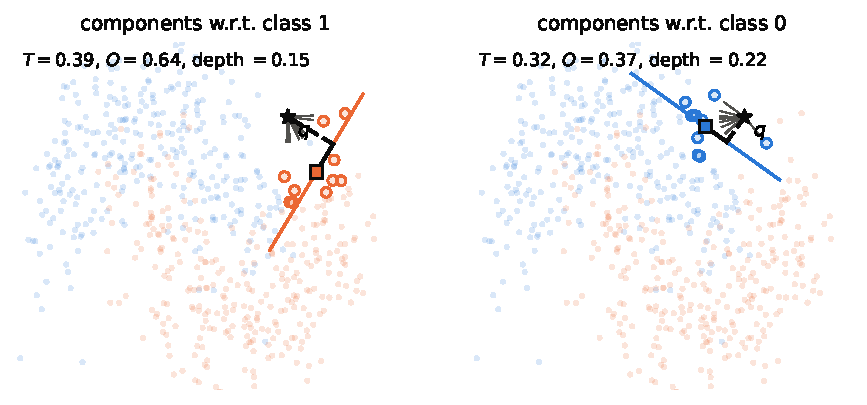
\includegraphics[width=0.56\linewidth]{../figures/decomposition.pdf}
\caption{The decomposition on the two-moons data for one query $q$ (star) with respect to each class: circles are the $k=10$ class neighbours, the square their centroid, the line the one-dimensional tangent subspace $T_1$; the solid segment is the tangential component, the dashed segment the orthogonal one; the short rays are the unit vectors $S(x_i-q)$ whose mean defines the spatial depth.}
\label{fig:schematic}
\end{figure}

Table~\ref{tab:main} gives the mean cross-validated accuracy of every method, Table~\ref{tab:delta} the primary comparison together with the comparison against \meth{HKNN}, and Table~\ref{tab:ablation} the ablations; Figure~\ref{fig:forest} shows the last two graphically. The comparison against every reference, the selective accuracies and the regime scan are tabulated in \path{results/tables_appendix.md}, generated by the same script as this document; the hyper-parameters are in Appendix~\ref{app:tables}. The whole experiment, including the regime scan, took \MetaSecondsCpu{} CPU-seconds.

\begin{table}[tb]
\centering\small\setlength{\tabcolsep}{3.6pt}
\begin{tabular}{lrrrrrrrrrrrrrr}
\toprule
& & & & \multicolumn{6}{c}{references} & \multicolumn{5}{c}{decomposition and ablations}\\
\cmidrule(lr){5-10}\cmidrule(lr){11-15}
dataset & $n$ & $d$ & $C$ & kNN & NFL & HKNN & LPH & LCD & SD & TOD & TO & TD & OD & T\\
\midrule
iris & 150 & 4 & 3 & 94.9 & 95.2 & 95.7 & \textbf{96.4} & 95.7 & 93.9 & 96.1 & 95.6 & 93.6 & 96.3 & 93.6 \\
wine & 178 & 13 & 3 & 96.3 & \textbf{97.0} & 97.0 & 95.9 & 96.9 & 96.4 & 97.1 & 96.9 & 96.4 & 97.3 & 89.5 \\
breast cancer & 569 & 30 & 2 & 96.6 & 96.0 & \textbf{97.0} & 96.7 & 96.9 & 95.5 & 96.7 & 97.1 & 95.7 & 96.7 & 93.3 \\
digits & 1000 & 64 & 10 & 96.4 & \textbf{97.6} & 97.4 & 97.4 & 96.9 & 91.0 & 97.2 & 97.3 & 92.1 & 97.1 & 43.6 \\
swiss roll & 600 & 3 & 3 & 96.8 & 92.9 & \textbf{97.4} & 97.0 & 96.9 & 95.4 & 97.2 & 97.2 & 95.2 & 97.1 & 78.9 \\
moons & 600 & 2 & 2 & 89.9 & 80.0 & \textbf{89.9} & 88.9 & 89.9 & 88.6 & 89.1 & 89.1 & 88.0 & 89.0 & 78.7 \\
moons+10 noise & 600 & 12 & 2 & 82.8 & 77.7 & \textbf{82.8} & 82.1 & 82.8 & 80.0 & 82.5 & 82.6 & 79.8 & 81.9 & 62.8 \\
spheres & 600 & 3 & 2 & 82.5 & 78.6 & \textbf{85.5} & 84.8 & 83.5 & 81.9 & 85.7 & 85.2 & 82.2 & 85.8 & 70.8 \\
\\
\bottomrule
\end{tabular}
\caption{Mean test accuracy (\%) over the \MetaFolds{} folds. The best reference on each dataset is in bold. TOD $=$ tangential $+$ orthogonal $+$ depth; TO, TD, OD drop one component; T, LPH ($=$O) and SD ($=$D) are the single components.}
\label{tab:main}
\end{table}

\begin{table}[tb]
\centering\footnotesize\setlength{\tabcolsep}{3.5pt}
\begin{tabular}{lllcccl}
\toprule
dataset & best ref. & TOD $-$ best [boot.\ CI] & NB CI & NB $p$ & W/L/T & TOD $-$ HKNN [boot.\ CI]\\
\midrule
iris & LPH & \ensuremath{-0.13} [\ensuremath{-1.07}, \ensuremath{+0.80}] & [\ensuremath{-2.86}, \ensuremath{+2.59}] & 0.920 & 5/5/15 & \ensuremath{+0.40} [\ensuremath{-0.27}, \ensuremath{+1.20}] \\
wine & HKNN & \ensuremath{-0.003} [\ensuremath{-1.25}, \ensuremath{+1.36}] & [\ensuremath{-3.86}, \ensuremath{+3.85}] & 0.999 & 5/8/12 & \ensuremath{-0.003} [\ensuremath{-1.25}, \ensuremath{+1.36}] \\
breast cancer & LCD & \ensuremath{-0.25} [\ensuremath{-0.71}, \ensuremath{+0.18}] & [\ensuremath{-1.56}, \ensuremath{+1.06}] & 0.700 & 5/8/12 & \ensuremath{-0.18} [\ensuremath{-0.63}, \ensuremath{+0.28}] \\
digits & NFL & \ensuremath{-0.36} [\ensuremath{-0.68}, \ensuremath{-0.06}] & [\ensuremath{-1.25}, \ensuremath{+0.53}] & 0.410 & 5/13/7 & \ensuremath{-0.16} [\ensuremath{-0.40}, \ensuremath{+0.08}] \\
swiss roll & HKNN & \ensuremath{-0.20} [\ensuremath{-0.60}, \ensuremath{+0.20}] & [\ensuremath{-1.34}, \ensuremath{+0.94}] & 0.721 & 7/9/9 & \ensuremath{-0.20} [\ensuremath{-0.60}, \ensuremath{+0.20}] \\
moons & kNN & \ensuremath{-0.77} [\ensuremath{-1.60}, \ensuremath{+0.20}] & [\ensuremath{-3.37}, \ensuremath{+1.84}] & 0.549 & 6/16/3 & \ensuremath{-0.70} [\ensuremath{-1.37}, \ensuremath{-0.03}] \\
moons+10 noise & LPH & \ensuremath{-0.33} [\ensuremath{-1.17}, \ensuremath{+0.47}] & [\ensuremath{-2.72}, \ensuremath{+2.06}] & 0.776 & 9/12/4 & \ensuremath{+0.23} [\ensuremath{-0.67}, \ensuremath{+1.13}] \\
spheres & HKNN & \ensuremath{+0.33} [\ensuremath{-0.43}, \ensuremath{+1.10}] & [\ensuremath{-1.87}, \ensuremath{+2.54}] & 0.758 & 12/10/3 & \ensuremath{+0.33} [\ensuremath{-0.43}, \ensuremath{+1.10}]
\\
\bottomrule
\end{tabular}
\caption{Primary comparison (C1), in accuracy points: mean and percentile bootstrap interval over the \MetaFolds{} folds, interval and $p$-value with the Nadeau--Bengio (NB) variance, folds won/lost/tied by TOD, and the same difference against HKNN. Significant wins under C1: \NSigWins{} of \NDatasets{} (\NRequired{} required; \NSigWinsNb{} with NB); significant losses: \NSigLosses{} with the bootstrap (\SigLossesList), \NSigLossesNb{} with NB.}
\label{tab:delta}
\end{table}

\paragraph{C1: the decomposition against the best reference.} The best reference was a local-support method (\meth{HKNN}, \meth{LPH} or \meth{NFL}) on \NBestRefHull{} of the \NDatasets{} datasets (Table~\ref{tab:delta}). \meth{TOD} beat it with a bootstrap interval above zero on \NSigWins{} of \NDatasets{} datasets, against \NRequired{} required; the criterion is not met. The mean difference ranged from \DeltaBestMin{} to \DeltaBestMax{} points (positive on \NDeltaPositive: \DeltaPositiveList) and was within one point on \NDeltaWithinOne{} of \NDatasets{} datasets; its bootstrap interval lay entirely below zero on \NSigLosses{} datasets (\SigLossesList): \DeltaBestTwoDigits{} points on digits [\CiLoBestTwoDigits, \CiHiBestTwoDigits] and \DeltaBestTwoMoons{} on moons [\CiLoBestTwoMoons, \CiHiBestTwoMoons]. Neither loss survives the corrected $t$-test ($p=\NbPBestDigits$ and $p=\NbPBestMoons$; NB intervals [\NbLoBestTwoDigits, \NbHiBestTwoDigits] and [\NbLoBestTwoMoons, \NbHiBestTwoMoons]), which is the cautious reading in both directions: the data neither show a gain nor establish a loss beyond a fraction of a point. The largest upper interval limit over all datasets is \CiHiBestMax{} points with the bootstrap and \CiHiBestMaxNb{} points with the Nadeau--Bengio variance (both on \CiHiBestMaxNbArg): gains larger than the latter are excluded at the 95\% level under the cautious reading, gains between the two values are excluded only under the anti-conservative one, and smaller gains are not excluded by this study.

\begin{table}[tb]
\centering\footnotesize\setlength{\tabcolsep}{4pt}
\begin{tabular}{lllll}
\toprule
dataset & $-$ depth (vs TO) & $-$ orthogonal (vs TD) & NB 95\% CI (vs TD) & $-$ tangential (vs OD)\\
\midrule
iris & $+0.5$ [-0.4, +1.5] & $+2.5$ [+1.3, +3.7] & [-0.9, +6.0] & $-0.1$ [-1.2, +0.8] \\
wine & $+0.2$ [-1.0, +1.5] & $+0.7$ [-0.6, +2.0] & [-3.2, +4.5] & $-0.2$ [-1.1, +0.7] \\
breast cancer & $-0.4$ [-0.7, -0.0] & $+1.1$ [+0.5, +1.7] & [-0.6, +2.7] & $+0.0$ [-0.5, +0.4] \\
digits & $-0.1$ [-0.3, +0.1] & $+5.1$ [+4.4, +5.8] & [+3.0, +7.2] & $+0.1$ [-0.1, +0.2] \\
swiss roll & $-0.1$ [-0.4, +0.3] & $+1.9$ [+1.2, +2.7] & [-0.2, +4.1] & $+0.1$ [-0.4, +0.5] \\
moons & $+0.0$ [-0.4, +0.4] & $+1.1$ [+0.2, +2.0] & [-1.5, +3.7] & $+0.1$ [-0.3, +0.6] \\
moons+10 noise & $-0.2$ [-1.1, +0.7] & $+2.7$ [+1.5, +3.8] & [-0.7, +6.0] & $+0.5$ [-0.4, +1.5] \\
spheres & $+0.5$ [-0.0, +1.0] & $+3.5$ [+2.3, +4.7] & [+0.0, +7.1] & $-0.1$ [-0.9, +0.7]
\\
\bottomrule
\end{tabular}
\caption{Ablations (C2): TOD minus the model with the named component removed, in accuracy points, mean and bootstrap 95\% interval; for the orthogonal component also the interval with the Nadeau--Bengio variance. A positive value means the component helped. Both intervals for all three ablations are in \texttt{results/tables\_appendix.md}.}
\label{tab:ablation}
\end{table}

\begin{figure}[tb]
\centering
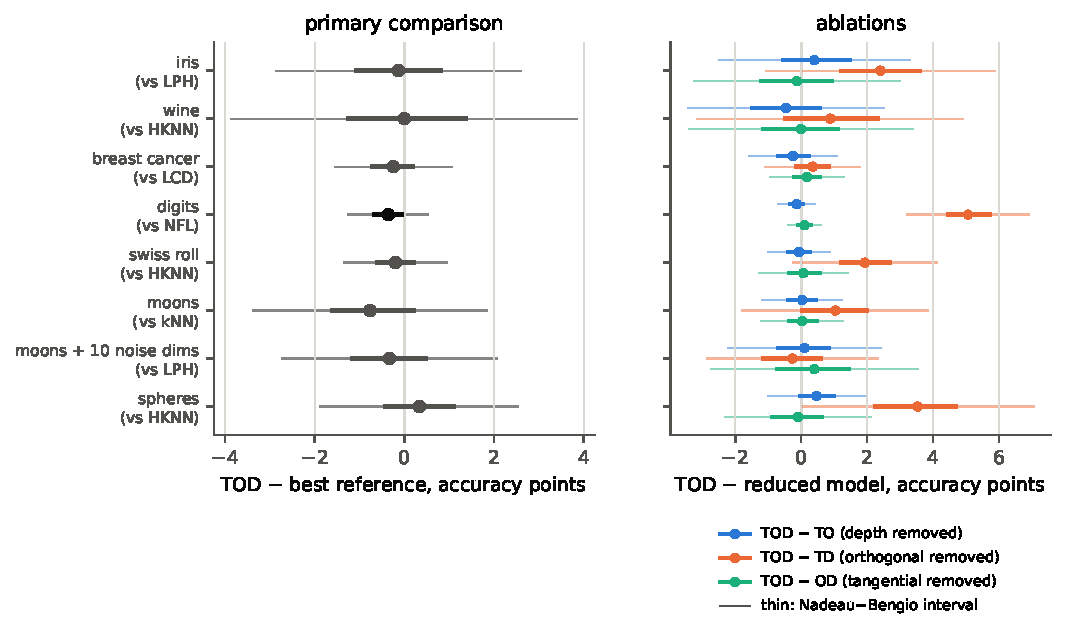
\includegraphics[width=0.78\linewidth]{../figures/forest.pdf}
\caption{Left: TOD minus the best reference per dataset (C1). Right: the three ablations (C2). Thick segments: bootstrap 95\% intervals; thin segments: intervals with the Nadeau--Bengio variance; black (left) marks a bootstrap interval excluding zero.}
\label{fig:forest}
\end{figure}

\paragraph{C2: where the information is.} Against \meth{HKNN}, the reference closest in spirit, the difference ranged from \DeltaHknnMin{} to \DeltaHknnMax{} points, with \NHknnCiAboveZero{} bootstrap intervals above zero and \NHknnCiBelowZero{} below (NB: \NHknnNbAboveZero{} and \NHknnNbBelowZero; Table~\ref{tab:delta}); against \meth{LPH} from \DeltaLphMin{} to \DeltaLphMax{} (\NLphCiAboveZero{} bootstrap interval above zero, \NLphNbAboveZero{} with NB). The one dataset on which \meth{TOD} beats the plain PCA hull with a bootstrap interval above zero is the spheres (\DeltaVsSpheresLph{} points; NB [\NbLoVsSpheresLph, \NbHiVsSpheresLph]), where the depth is the component that helps (\meth{TOD} $-$ \meth{TO} $=$ \AblSpheresTo{} [\AblLoSpheresTo, \AblHiSpheresTo]); but \meth{HKNN} closes the same gap with its penalty, and \meth{TOD} $-$ \meth{HKNN} is \DeltaVsSpheresHknn{} points there. \meth{TOD} beat \meth{kNN} with a bootstrap interval above zero on \NKnnCiAboveZero{} datasets (\NKnnNbAboveZero{} with NB) and the depth-only classifier \meth{SD} on \NSdCiAboveZero{} of \NDatasets{} (\NSdNbAboveZero{} with NB); the hull classifiers do the same, so these are the known advantages of local hulls over points and over depth~\citep{vincentbengio2002}, not a contribution of the decomposition. The accuracies of \meth{HKNN}, \meth{LPH}, \meth{TOD}, \meth{TO} and \meth{OD} never differ by more than \HullFamilyMaxSpread{} points on any dataset: they behave as one family, as Proposition~\ref{prop:hknn} and Remark~\ref{rem:family} suggest.

The ablations (Table~\ref{tab:ablation}, Figure~\ref{fig:forest}) say where the information sits. Removing the orthogonal component costs between \AblOrthMin{} and \AblOrthMax{} points, with a bootstrap interval above zero on \NAblOrthCiAboveZero{} of \NDatasets{} datasets and a Nadeau--Bengio interval above zero on \NAblOrthNbAboveZero{} (\AblOrthNbAboveList); the attribution therefore rests on the size of the effects (\AblDigitsTd{} points on digits, \AblSpheresTd{} on spheres, \AblMoonsNTd{} on the moons with noise) and on the fitted weights, not on a count of intervals. Removing the depth changes accuracy by \AblDepthMin{} to \AblDepthMax{} points, with \NAblDepthCiAboveZero{} bootstrap intervals above zero and \NAblDepthCiBelowZero{} below (breast cancer, upper limit \AblHiBcTo, i.e.\ marginal; \NAblDepthNbAboveZero{} and \NAblDepthNbBelowZero{} with NB); removing the tangential component changes it by \AblTangMin{} to \AblTangMax{} points, with \NAblTangCiAboveZero{} and \NAblTangCiBelowZero{} bootstrap intervals above and below zero (\NAblTangNbAboveZero{} and \NAblTangNbBelowZero{} with NB). The largest upper limits for the depth and tangential contributions are \AblDepthCiHiMax{} and \AblTangCiHiMax{} points with the bootstrap, \AblDepthNbHiMax{} and \AblTangNbHiMax{} with NB. The fitted weights tell the same story (Table~\ref{tab:params}, Appendix~\ref{app:tables}): the weight on $\log O$ lies between \WOMin{} and \WOMax{} across datasets, the weight on $\log T$ between \WTMin{} and \WTMax, and the weight on $\log E$ between \WDMin{} and \WDMax, negative on \NWDNegative{} datasets, so its sign is not even stable. The tangential distance alone is a poor classifier (\meth{T}: from \AccTMin\% on \AccTArgMin{} to \AccTMax\%), consistent with it being a within-support coordinate rather than an off-support one.

\paragraph{C3: abstention.} With each method abstaining on its own least confident fifth of the test points, \meth{TOD} differed from the best reference of Table~\ref{tab:delta} by \SelDeltaMin{} to \SelDeltaMax{} points; the bootstrap interval lay above zero on \NSelCiAboveZero{} dataset (digits, \SelDeltaBestDigits{} points; NB [\SelNbLoDigits, \SelNbHiDigits]) and below zero on \NSelCiBelowZero{} (moons and moons with noise, \SelDeltaBestMoons{} and \SelDeltaBestMoonsN); with NB, \NSelNbAboveZero{} above and \NSelNbBelowZero{} below. The natural comparison for abstention is with the reference that is best \emph{by selective accuracy}: there the differences run from \SelBySelDeltaMin{} to \SelBySelDeltaMax{} points with \NSelBySelCiAboveZero{} bootstrap intervals above zero and \NSelBySelCiBelowZero{} below (\SelBySelBelowList); on digits that reference is \meth{\SelBySelRefDigits} and the difference is \SelBySelDeltaDigits{} [\SelBySelLoDigits, \SelBySelHiDigits]. The posterior of the three-component logit is therefore not a better abstention signal than the margins of the reference scores; in particular the depth, which one might expect to flag off-support queries, does not improve selective accuracy here.

\begin{figure}[tb]
\centering
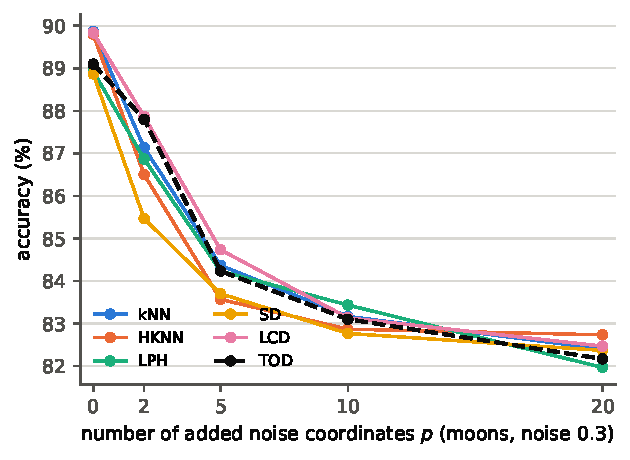
\includegraphics[width=0.4\linewidth]{../figures/regime.pdf}
\caption{E2: accuracy against the number $p$ of appended noise coordinates for five references and TOD (dashed); the best reference at each $p$ is the highest line (\RegBestSet).}
\label{fig:regime}
\end{figure}

\paragraph{E2: the off-manifold-noise regime.} Appending noise coordinates to the moons lowers every method (Figure~\ref{fig:regime}; table in \path{results/tables_appendix.md}): \meth{kNN} by \RegKnnDrop{} points from $p=0$ to $p=20$, \meth{HKNN} by \RegHknnDrop, \meth{TOD} by \RegTodDrop, \meth{SD} by \RegSdDrop. The best reference at each $p$ was one of \{\RegBestSet\}; \meth{TOD} minus the best reference ranged from \RegDeltaMin{} to \RegDeltaMax{} points with \NRegSigWins{} bootstrap intervals above zero and \NRegSigLosses{} below (\NRegSigWinsNb{} and \NRegSigLossesNb{} with NB). The depth contribution (\meth{TOD} $-$ \meth{TO}) ranged from \RegAblDepthMin{} to \RegAblDepthMax{} points and the tangential contribution (\meth{TOD} $-$ \meth{OD}) from \RegAblTangMin{} to \RegAblTangMax, with \NRegAblDepthCiAboveZero{} and \NRegAblTangCiAboveZero{} bootstrap intervals above zero respectively; the orthogonal contribution (\meth{TOD} $-$ \meth{TD}) ranged from \RegAblOrthMin{} to \RegAblOrthMax. The single bootstrap interval above zero for the depth contribution in the whole study occurs at $p=2$ (\RegAblDepthPTwo{} points [\RegAblDepthLoPTwo, \RegAblDepthHiPTwo]; NB [\RegAblDepthNbLoPTwo, \RegAblDepthNbHiPTwo], $p=\RegAblDepthNbPPTwo$). It is one of \NDepthIntervals{} depth intervals examined in E1 and E2 (the $p=0$ row repeats the moons), so it is compatible with chance even before the dependence between folds is taken into account, and there \meth{TOD} remains \RegDeltaPTwo{} points from the best reference (\RegBestPTwo, \RegBestAccPTwo\%): with a few noise coordinates the depth helps the logit model catch up with the references, not overtake them. There is thus no noise regime, in this range, in which the depth or the tangential component adds to what the best reference already achieves.

\section{What can be claimed}\label{sec:claims}

\begin{table}[tb]
\centering\small
\begin{tabular}{p{0.76\linewidth}l}
\toprule
claim & status\\
\midrule
C1: TOD beats the best reference on \NSigWins{} of \NDatasets{} datasets (\NRequired{} required; \NSigWinsNb{} with NB); the decomposition \VerdictWord{} information in the predefined sense & verified (negative)\\
Upper 95\% limit of the gain over the best reference: at most \CiHiBestMax{} points (bootstrap) / \CiHiBestMaxNb{} points (NB) on every dataset & verified\\
C2: the orthogonal component carries the information: removing it costs \AblOrthMin{} to \AblOrthMax{} points (interval above zero on \NAblOrthCiAboveZero/\NDatasets{} bootstrap, \NAblOrthNbAboveZero/\NDatasets{} NB); depth and tangential components removable without significant loss (\NAblDepthCiAboveZero/\NDatasets{} and \NAblTangCiAboveZero/\NDatasets{} bootstrap, \NAblDepthNbAboveZero/\NDatasets{} and \NAblTangNbAboveZero/\NDatasets{} NB) & verified\\
C3: no gain in selective accuracy at \MetaCoverage\% coverage (\NSelCiAboveZero{} bootstrap interval above zero against the best reference by accuracy, \NSelBySelCiAboveZero{} against the best by selective accuracy, \NSelNbAboveZero{} with NB) & verified\\
E2: no off-manifold-noise regime with $p\le20$ in which TOD exceeds the best reference; the depth helps the logit model only at $p=2$ (\RegAblDepthPTwo{} points, bootstrap; NB $p=\RegAblDepthNbPPTwo$) & verified\\
HKNN, LPH, TOD, TO, OD differ by at most \HullFamilyMaxSpread{} points on every dataset & verified\\
Gains below \CiHiBestMaxNb{} points (below \CiHiBestMax{} under the bootstrap); behaviour on large or high-dimensional data; other depths & not established\\
\bottomrule
\end{tabular}
\caption{Empirical claims and their status; the propositions of Section~\ref{sec:theory} are labelled where they are stated. ``Verified'' means produced by the scripts of Appendix~\ref{app:repro} with the fixed seed on the datasets of Section~\ref{sec:protocol}; it is not a general statement.}
\label{tab:claims}
\end{table}

Table~\ref{tab:claims} lists the claims with their status. The answer to the line's question, in the operational sense fixed in Section~\ref{sec:protocol}, is negative: the tangential--orthogonal--depth decomposition does not add predictive information beyond the local hull. Proposition~\ref{prop:hknn} says why the tangential part cannot be expected to: the regularised hull distance already contains it with a sensible weighting. The depth was formally free to help (Proposition~\ref{prop:nonredundant}) and did not add to the best reference, in accuracy or in abstention, on any of the \NDatasets{} datasets or in the noise regime scanned; its one bootstrap-significant contribution ($p=2$ in E2, not significant with the Nadeau--Bengio variance) brought the logit model level with the references, not past them.

\paragraph{Limitations.} The datasets are small and, for \NNearCeiling{} of them (\NearCeilingList), the best reference is at or above 96\% accuracy, close to the ceiling; one test error is worth \FoldResIris{} accuracy points on iris and \FoldResWine{} on wine, so ``within one point'' is there below the resolution of a single fold and most folds are exact ties (W/L/T in Table~\ref{tab:delta}). The study therefore has power to exclude gains of a few points, \CiHiBestMaxNb{} with the Nadeau--Bengio variance and \CiHiBestMax{} with the fold-level bootstrap, which is anti-conservative because the folds of repeated cross-validation share data; it does not exclude smaller gains. Every count of significant differences is given in both readings, and the attribution of C2 rests on effect sizes rather than on counts. Hyper-parameters were chosen by leave-one-out accuracy on the training fold and the logit weights were fitted on the same leave-one-out features, an optimism of three parameters shared by all logit models; the references have one or two tuned parameters each. On the moons and the moons with noise the chosen neighbourhood size sits at the top of the grid in most folds for both \meth{TOD} and \meth{HKNN} (Section~\ref{sec:protocol}). Only one depth (local spatial depth) and one combination rule (a conditional logit without intercepts) were tried; a different depth, per-class weights or a non-linear combiner could behave differently, and the negative finding is about the tested instance, not about every conceivable use of the components. The tangent dimension $m$ was tuned globally, not per neighbourhood by explained variance. No class priors are used by the score-based methods, which handicaps them slightly on the imbalanced breast-cancer data relative to \meth{kNN}.

\paragraph{Next steps for the research line.} The line's stated objective is discharged with a negative answer and can be closed. If it were reopened, the only directions the present results leave open are: (a) depths with a different mechanism (halfspace or simplicial depth on the neighbourhood, or the symmetrised local depth of \citealp{paindaveinevanbever2013}) tested under the same criterion; (b) the use of the decomposition as a \emph{descriptive} tool for local-hull methods, e.g.\ choosing $\lambda$ from the spectrum $(s_j)$ via Proposition~\ref{prop:hknn} rather than by search, which is a question about HKNN and not about a new classifier; (c) larger and higher-dimensional data, where the hull methods differ more from \meth{kNN} and the hull distance is not identically zero (Remark~\ref{rem:lowdim}), with the caveat that the study would then be about the hull family and not about the added components.

\appendix
\section{Reproducibility}\label{app:repro}
{\sloppy The directory contains \path{experiments/support_geometry.py} (the whole experiment, E1 and E2; flag \texttt{--fast} for a reduced run), \path{experiments/make_figures.py} and \path{experiments/make_numbers.py}, which converts \path{results/results.json} and \path{results/results_regime.json} into the macros and table bodies used by this document and into \path{results/tables_appendix.md}, so that every number in the text is generated and none is typed; the Nadeau--Bengio intervals, the grid-edge fractions and the modal hyper-parameters are recomputed by that script from the per-fold lists. The run used seed \MetaSeed, Python \MetaPython, NumPy \MetaNumpy~\citep{harris2020}, SciPy \MetaScipy~\citep{virtanen2020} and scikit-learn \MetaSklearn~\citep{pedregosa2011}, single-threaded BLAS, and took \MetaSecondsWall{} s wall / \MetaSecondsCpu{} s CPU on a shared four-core machine. The first run with the narrower grids is kept as \path{results/tables_run1_narrow_grids.md}. Computation: per fold, all squared distances are computed once; for each class and $k$ the $k$ nearest same-class points are found by partial sorting and decomposed by a batched thin SVD, from which all scores and the closed form of Proposition~\ref{prop:hknn} are evaluated (checked against brute force and \texttt{lstsq} before the runs); logit weights are fitted by L-BFGS-B with the analytic gradient.\par}

\section{Hyper-parameters}\label{app:tables}
\begin{table}[htb]
\centering\footnotesize\setlength{\tabcolsep}{3.5pt}
\begin{tabular}{lrrrrrcrrr}
\toprule
dataset & $\kNN$ & HKNN $(k,\lambda_{\rm rel})$ & LPH $(k,m)$ & SD $k$ & TOD $(k,m)$ & \shortstack{\% folds at $k{=}\MetaKMax$\\(TOD / HKNN)} & $w_T$ & $w_O$ & $w_D$\\
\midrule
iris & 11 & (30, 0.1) & (20, 2) & 10 & (20, 2) & 0.82 & 2.95 & 1.40 \\
wine & 31 & (30, 1) & (20, 2) & 20 & (30, 8) & 1.38 & 3.09 & 1.81 \\
breast cancer & 3 & (20, 10) & (20, 1) & 20 & (20, 1) & 0.71 & 2.91 & 0.89 \\
digits & 1 & (20, 0.1) & (10, 8) & 10 & (10, 8) & 0.29 & 3.93 & 0.52 \\
swiss roll & 5 & (5, 1) & (5, 1) & 10 & (10, 1) & 0.17 & 3.30 & 0.57 \\
moons & 41 & (30, 10) & (20, 1) & 30 & (30, 1) & 0.42 & 1.52 & -0.12 \\
moons+10 noise & 41 & (30, 100) & (30, 1) & 30 & (30, 5) & 0.37 & 3.04 & -1.15 \\
spheres & 7 & (5, 10) & (5, 1) & 10 & (10, 1) & 0.26 & 1.92 & -0.53
\\
\bottomrule
\end{tabular}
\caption{Modal hyper-parameters over the \MetaFolds{} folds (ties towards the smallest values), the percentage of folds in which the chosen neighbourhood size is the largest in the grid, and the mean fitted weights of TOD on the standardised features $\log T_m$, $\log O_m$, $\log E$ (larger weight $=$ more influence; positive $=$ smaller value favours the class).}
\label{tab:params}
\end{table}

\renewcommand{\bibfont}{\footnotesize}
\setlength{\bibsep}{2.5pt}
\bibliographystyle{plainnat}
\bibliography{refs}
\end{document}
